\documentclass[twocolumn,english]{IEEEtran}
\usepackage[T1]{fontenc}
\usepackage{babel}
\usepackage{amsthm}
\usepackage{amsmath}
\usepackage{graphicx}
\usepackage[unicode=true,
 bookmarks=true,bookmarksnumbered=true,bookmarksopen=true,bookmarksopenlevel=1,
 breaklinks=false,pdfborder={0 0 0},backref=false,colorlinks=false]
 {hyperref}
\usepackage{bm}
\usepackage{amsmath}
\usepackage{amssymb}
\usepackage{natbib}
\usepackage{array}
\usepackage{calc}
\newcommand{\vb}[1]{\mathbf{#1}}		%Bold vector
\newcolumntype{W}{>{\centering\arraybackslash}m{25mm}}
\newcolumntype{L}{>{\centering\arraybackslash}m{15mm}}
\usepackage{booktabs}

%%%%%%%%%%%%%%%%%%%%%%%%%%%%%%%%%%%%%%%%%%%%%%%%%%%%%%%%%%%%%%%%%%%%%%%%%%%%%%% Variables
\newcommand{\thetitle}{Project 1: Descriptive Statistics}
\newcommand{\theauthors}{Zack Garza}
\newcommand{\theclass}{Math 142: Elementary Statistics}
%%%%%%%%%%%%%%%%%%%%%%%%%%%%%%%%%%%%%%%%%%%%%%%%%%%%%%%%%%%%%%%%%%%%%%%%%%%%%%%%%%%%%%%%%%

\hypersetup{
 pdftitle=  {\thetitle},
 pdfauthor= {\theauthors},
 pdfpagelayout=OneColumn, pdfnewwindow=true, pdfstartview=XYZ, plainpages=false}

\makeatletter


%%%%%%%%%%%%%%%%%%%%%%%%%%%%%% Textclass specific LaTeX commands.
 % protect \markboth against an old bug reintroduced in babel >= 3.8g
 \let\oldforeign@language\foreign@language
 \DeclareRobustCommand{\foreign@language}[1]{%
   \lowercase{\oldforeign@language{#1}}}
\theoremstyle{plain}
\newtheorem{thm}{\protect\theoremname}
\theoremstyle{plain}
\newtheorem{lem}[thm]{\protect\lemmaname}

%%%%%%%%%%%%%%%%%%%%%%%%%%%%%% User specified LaTeX commands.
% for subfigures/subtables
\ifCLASSOPTIONcompsoc
\usepackage[caption=false,font=normalsize,labelfont=sf,textfont=sf]{subfig}
\else
\usepackage[caption=false,font=footnotesize]{subfig}
\fi

\makeatother
\providecommand{\lemmaname}{Lemma}
\providecommand{\theoremname}{Theorem}
\setcounter{topnumber}{2}
\setcounter{bottomnumber}{2}
\setcounter{totalnumber}{4}
\renewcommand{\topfraction}{0.85}
\renewcommand{\bottomfraction}{0.85}
\renewcommand{\textfraction}{0.15}
\renewcommand{\floatpagefraction}{0.7}
\usepackage{float}
\onecolumn

\usepackage{Sweave}
\begin{document}

\title{\thetitle}
\author{\theauthors}
\IEEEspecialpapernotice
{\theclass \\ Effective Date of Report: \today }
\markboth{\thetitle}{\theauthors}
\maketitle
\tableofcontents

\hrulefill

\section{Part 1}
The data set used for this analysis is ``Data Set 8: Alcohol and Tobacco Use in Animated Children's Movies'' from Appendix B in \textit{Elementary Statistics} by Triola. The data analyzed were the movie lengths in seconds.

Figure 1 shows the frequency distribution of the movie lengths.

\begin{figure}[h!]
\begin{centering}
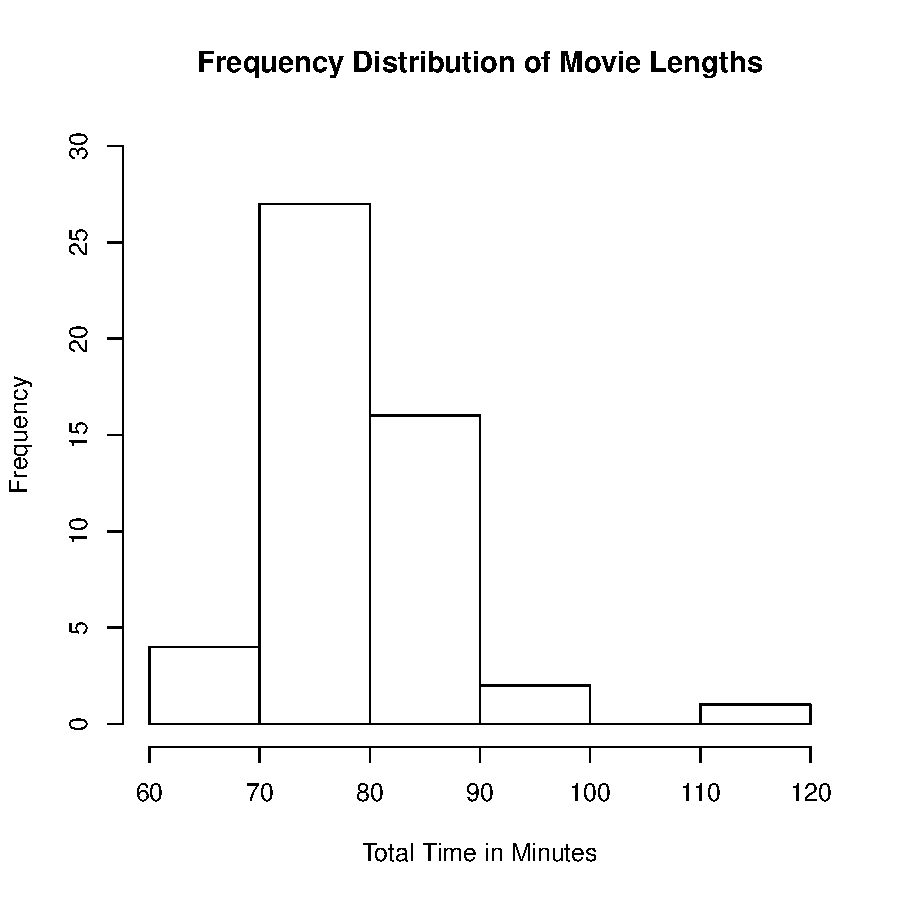
\includegraphics{proj1-fig1}
\caption{Running Times of a Sample of G-Rated movies.}
\label{fig:one}
\end{centering}
\end{figure}

\newpage

\section{Measures of Center}
\begin{Schunk}
\begin{Soutput}
Mean:  79.2
\end{Soutput}
\begin{Soutput}
Median:  77.5
\end{Soutput}
\begin{Soutput}
Mode:  75
\end{Soutput}
\begin{Soutput}
Midrange:  92
\end{Soutput}
\begin{Soutput}
Range:  56
\end{Soutput}
\begin{Soutput}
Sample Standard Deviation:  8.962507
\end{Soutput}
\end{Schunk}

\noindent \hrulefill\\
\noindent \textbf{5 Number Summary:}
\begin{Schunk}
\begin{Soutput}
   Min. 1st Qu.  Median    Mean 3rd Qu.    Max. 
  64.00   74.00   77.50   79.20   82.75  120.00 
\end{Soutput}
\end{Schunk}
\noindent \hrulefill

\section{Modified Box Plot}
Quantiles:
\begin{Schunk}
\begin{Soutput}
    0%    25%    50%    75%   100% 
 64.00  74.00  77.50  82.75 120.00 
\end{Soutput}
\end{Schunk}

\begin{figure}[h!]
\begin{centering}
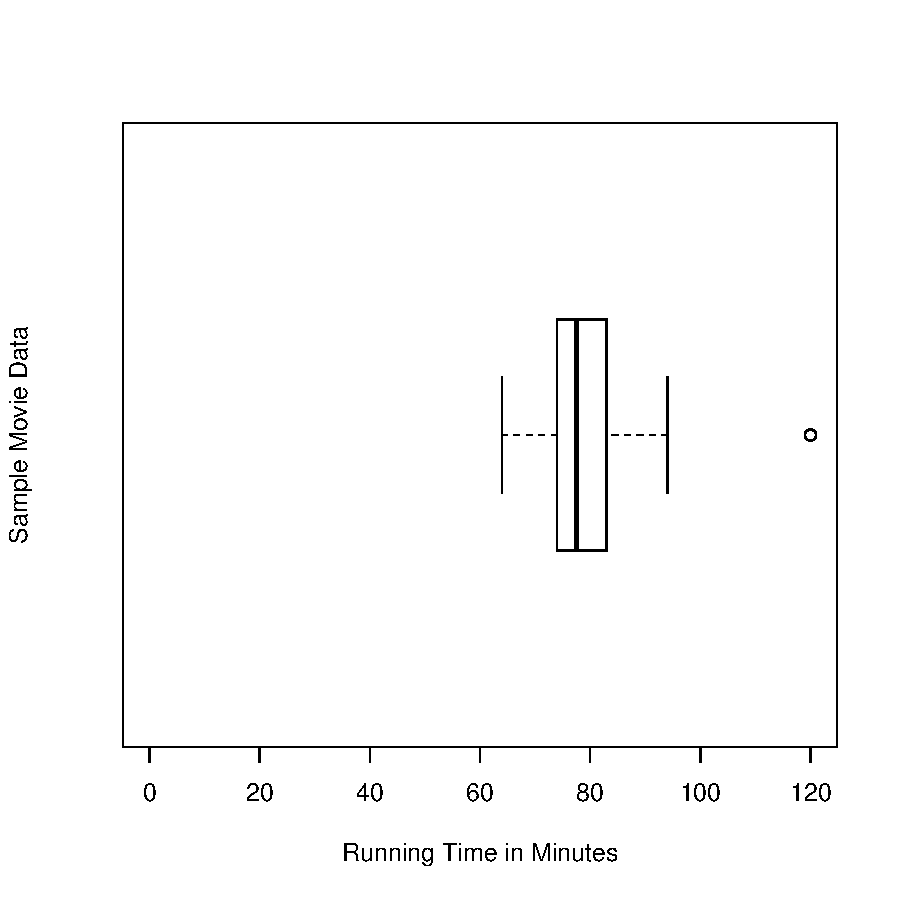
\includegraphics{proj1-boxplot1}
\caption{Modified Box Plot}
\label{fig:one}
\end{centering}
\end{figure}

%\appendices{}
%\bibliographystyle{plain}
%\bibliography{physbib}

\end{document}
